\documentclass[10pt]{minimal}

\usepackage[latin1]{inputenc}
\usepackage{tikz}
\usetikzlibrary{shapes,arrows, fit}
\begin{document}
\pagestyle{empty}


% Define block styles
\tikzstyle{block} = [rectangle, draw, fill=blue!20, 
    text width=10em, text centered, minimum height=3em,line width=.3mm]
\tikzstyle{line} = [draw, -latex', line width=.5mm]
\tikzstyle{cloud} = [draw, rounded rectangle,fill=red!20, text width=7em, text centered,
    minimum height=4em,line width=.3mm]
    \tikzstyle{input} = [draw, rounded rectangle,fill=green!20, text width=7em, text centered,
    minimum height=4em, line width=.3mm]
    
\begin{tikzpicture}[node distance =3cm]
\node [input] (freq) {Frequency source};
\node [input, right of=freq, xshift=0cm] (dict) {Dictionary};
\node [block, text width=13em, below of=freq, yshift=0cm, xshift=2cm] (dist) {Filter for valid distractors:\\ a) in frequency source \\ b) only lowercase alpha characters \\ c) not on manual exclude list \\ d) in model vocab };
\node [cloud, text width =12em, below of=dist, xshift=0cm, yshift=0cm] (distlist) {(Length, frequency) : potential distractors\\ lookup };
     
 \node [input, left of=freq, xshift=-6.5cm, yshift=2.5cm, line width=.5mm] (mat) {\textbf{Materials}};
   \node [block, below of =mat, xshift=.5cm, yshift=1cm] (prep) {Read in materials};
 \node [block, below right of=prep,xshift=-.4cm, yshift=0cm] (sentence) {Incrementally model sentence};     
   \node [input, right of=mat,xshift=1cm, yshift=-.5cm, text width=10em] (NN) {Neural Net model\\{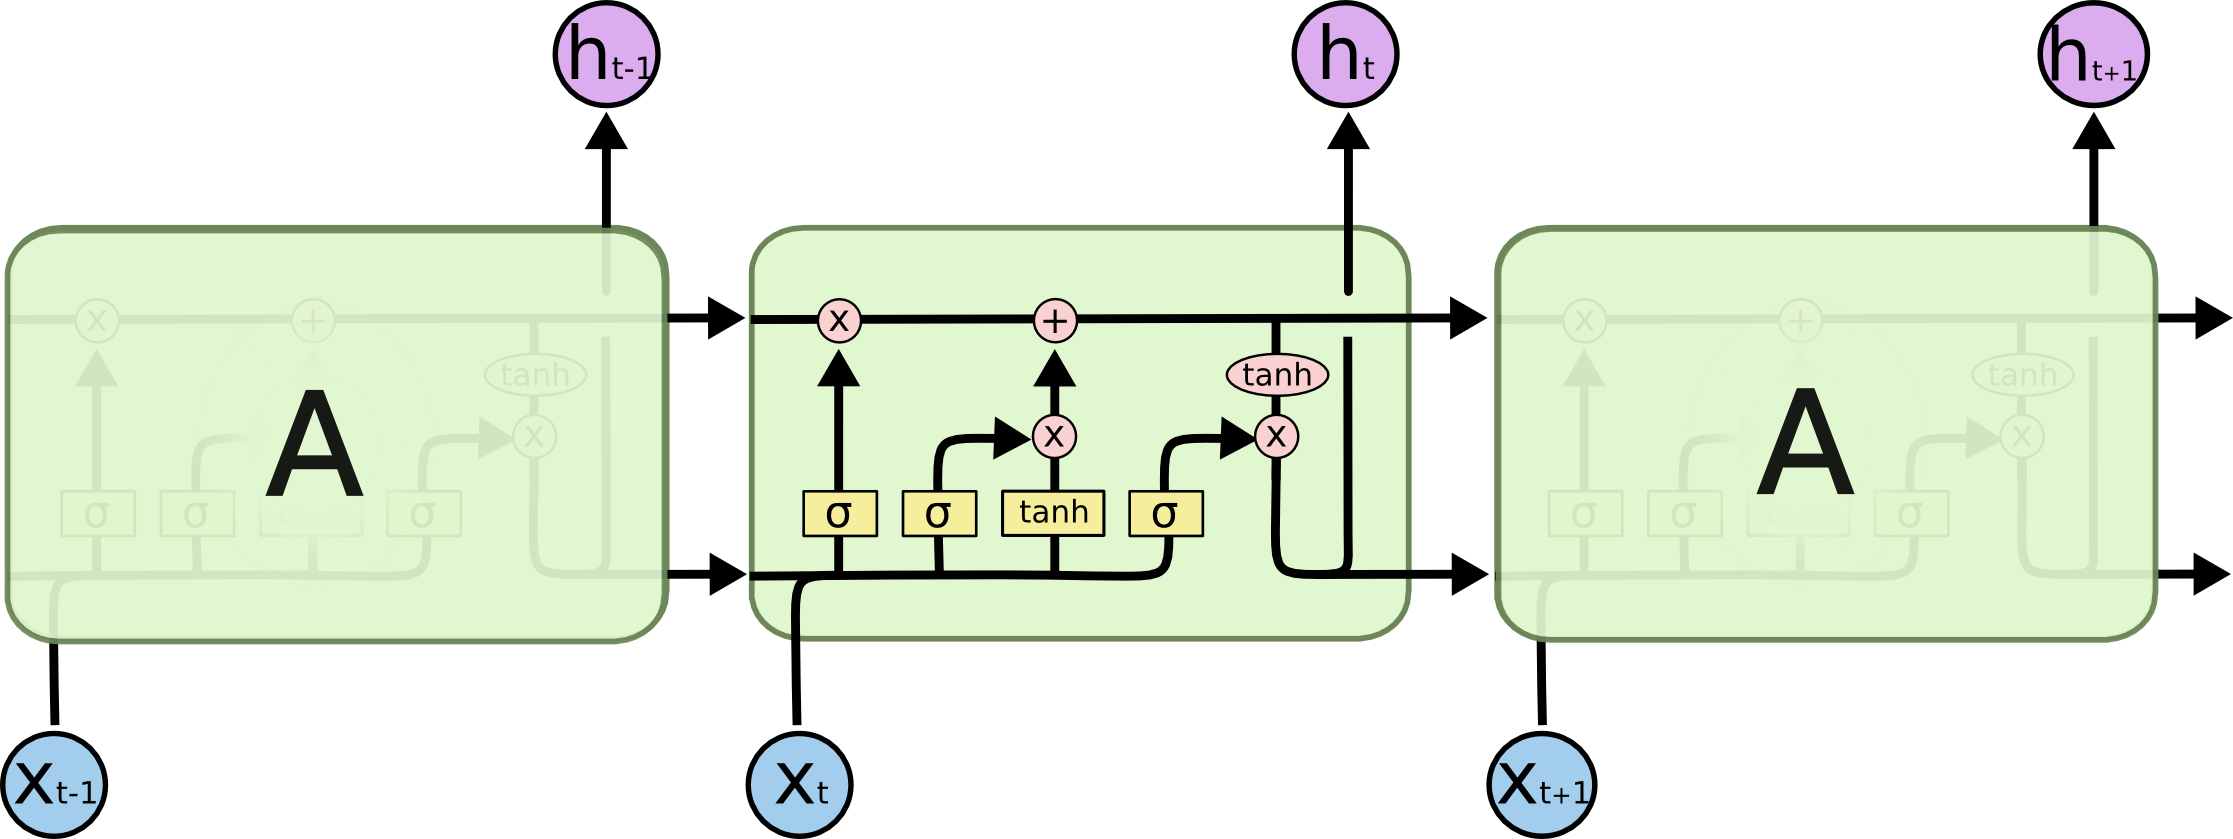
\includegraphics[width=3cm]{lstm.png}}};   

   \node [cloud, below right of=sentence, xshift=.5cm,  yshift=0cm] (word2) {True next word};  
\node [cloud, below left of =sentence, xshift=.5cm,  yshift=0cm] (surp) {Probability distribution over next word};
\node [block, below  of =word2, yshift=1cm, xshift=-.5cm] (potdist) {Generate length, frequency matched potential distractors};
\node [block, text width=12em,  below of =potdist, yshift=1cm, xshift=-3cm] (choose) {Choose  distractor word with high  surprisal};
\node [cloud, below of =choose, xshift=-1cm, yshift=1cm] (distractor) {Distractor};

\node [block, right of =distractor, xshift=1cm] (collect) {Collect distractor words into a sentence};

\node [block, right of =choose, xshift=5cm] (format) {Write items and distractors to file};

\node [input, line width= .5mm, below of=format, yshift=1cm] (final) {\textbf{Materials for Maze experiment}};
\node[draw,dotted, line width= .5mm, fit=(freq) (distlist) (dict) (dist)] (box1) { };
\node[draw, draw=none, above of=box1, xshift=0cm,  yshift=1cm] {Set up};
\node[draw,dashed,blue,line width=.5mm, inner sep=10pt, fit= (surp) (word2)(choose)(potdist)] (box2){ };
\node[draw, draw=none, above of=box2, xshift=0cm,  yshift=.2cm] {Do for each word in sentence};
	\node[draw,dashed,red,line width=.5mm, inner sep=13pt, fit= (word2) (surp) (choose) (distractor) (collect)  (sentence)] (box3) { };
\node[draw, draw=none, above of=box3, xshift=0cm,  yshift=2.4cm] {Do for each item in materials};
    % Draw edges
    \path [line] (dict) -- (dist);
    \path [line] (dist.south) -- (distlist.north);
	\path [line] (word2) -- (potdist);
	\path [line] (freq) -- ([yshift=.2cm]potdist.east);
		\path [line] (freq) -- (dist);
	\path [line] (distlist) -- (potdist);
	\path [line] (potdist) -- (choose);	
	\path [line] (surp) -- (choose);
	\path [line] (choose) -- (distractor);
	\path [line] ([yshift=-.2cm]sentence) -| ([xshift=-.7cm]surp.north);
	\path [line] ([yshift=-.2cm]sentence) -| ([xshift=.7cm]word2.north);
	\path [line] ([xshift=-1cm]prep.south) |- ([yshift=.2cm]sentence.west);
	\path [line] ([xshift=1.5cm]NN.south) |- ([yshift=.2cm]sentence.east);
	\path [line] (distractor) -- (collect);
	\path [line] (collect) -- (format.west);
	\path [line] (format) -- (final);
	\path [line] (mat) -- (prep);


\end{tikzpicture}


\end{document}